\documentclass[times,specification,annotation]{itmo-student-thesis}

%% Опции пакета:
%% - specification - если есть, генерируется задание, иначе не генерируется
%% - annotation - если есть, генерируется аннотация, иначе не генерируется
%% - times - делает все шрифтом Times New Roman, собирается с помощью xelatex
%% - pscyr - делает все шрифтом Times New Roman, требует пакета pscyr.

%% Делает запятую в формулах более интеллектуальной, например:
%% $1,5x$ будет читаться как полтора икса, а не один запятая пять иксов.
%% Однако если написать $1, 5x$, то все будет как прежде.
\usepackage{icomma}

\graphicspath{ {./img/} }

%% Один из пакетов, позволяющий делать таблицы на всю ширину текста.
\usepackage{tabularx}

%% Данные пакеты необязательны к использованию в бакалаврских/магистерских
%% Они нужны для иллюстративных целей
%% Начало
\usepackage{tikz}
\usetikzlibrary{arrows}
\usepackage{filecontents}

%% Указываем файл с библиографией.
\addbibresource{bachelor-thesis.bib}

\begin{document}

\studygroup{M3436}
\title{Rendering atmospheric clouds using neural networks}
\author{Панин Михаил Иванович}{Панин М.И.}
\supervisor{Ковалёв Антон Сергеевич}{Ковалёв А.С.}{доцент}{ФИТиП}
\publishyear{2019}
%% Дата выдачи задания. Можно не указывать, тогда надо будет заполнить от руки.
\startdate{01}{сентября}{2018}
%% Срок сдачи студентом работы. Можно не указывать, тогда надо будет заполнить от руки.
\finishdate{31}{мая}{2019}
%% Дата защиты. Можно не указывать, тогда надо будет заполнить от руки.
\defencedate{15}{июня}{2019}

\addconsultant{Николенко С.И.}{канд. физ.-мат. наук, зав. Лаб. искусственного интеллекта ПОМИ РАН}

\secretary{Павлова О.Н.}

%% Задание
%%% Техническое задание и исходные данные к работе
\technicalspec{Требуется реализовать метод рендеринга облаков "Deep Scattering" от Disney. На основании него разработать более производительный метод. Провести сравнительный анализ производительности и качества рендеринга.}

%%% Содержание выпускной квалификационной работы (перечень подлежащих разработке вопросов)
\plannedcontents{Изучить метод рендеринга облаков "Deep Scattering". Реализовать рендеринг облаков с помощью метода Монте-Карло для контроля результатов и сбора датасета. Собрать датасет из 15 млн элементов. Реализовать метод "Deep Scattering". Проэксперементировать с архитектурами нейронной сети и найти более производительный вариант, выдающий качественный результат.}

%%% Исходные материалы и пособия 
\plannedsources{Графические материалы и чертежи работой не предусмотрены}

%%% Цель исследования
\researchaim{Раработка нового, более эффективного метода рендеринга облаков.}

%%% Задачи, решаемые в ВКР
\researchtargets{\begin{enumerate}
    \item Реализовать рендеринг облаков с помощью метода Монте-Карло;
    \item Собрать датасет из 15 млн элементов;
    \item Реализовать метод рендеринга "Deep Scattering";
    \item Разработать более производительный метод, выдающий фотореалистичный результат;
\end{enumerate}}

%%% Использование современных пакетов компьютерных программ и технологий
\addadvancedsoftware{\texttt{NVIDIA® OptiX™} для трассировки лучей на видеокарте}{TODO: ref}
\addadvancedsoftware{Компилятор \texttt{NVIDIA CUDA} для вычислений на видеокарте}{TODO: ref}
\addadvancedsoftware{Библиотека \texttt{protobuf} для эффективной сериализации датасета}{TODO: ref}
\addadvancedsoftware{База данных \texttt{LMDB} для хранения датасета}{TODO: ref}
\addadvancedsoftware{Фреймворк \texttt{PyTorch} для обучения и экспорта нейронной сети}{TODO: ref}
\addadvancedsoftware{Среда разработки \texttt{Microsoft Visual Studio} для разработки на \texttt{C++}}{TODO: ref}
\addadvancedsoftware{Среда разработки \texttt{PyCharm} для разработки на \texttt{Python}}{TODO: ref}

%%% Краткая характеристика полученных результатов 
\researchsummary{Собран датасет облаков. Представлен новый метод рендеринга, превосходящий по производительности "Deep Scattering".}

%%% Гранты, полученные при выполнении работы 
\researchfunding{Грантов получено не было}

%%% Наличие публикаций и выступлений на конференциях по теме выпускной работы
\researchpublications{Публикаций не было}

%% Эта команда генерирует титульный лист и аннотацию.
\maketitle{Бакалавр}

%% Оглавление
\tableofcontents

%% Макрос для введения. Совместим со старым стилевиком.
\startprefacepage

Physically correct rendering of atmospheric clouds was always a difficult task to solve. Even with today's computing power, rendering a 1920x1080 image of a cloud using monte-carlo path tracing, takes a day or two to complete. 

Various optimizations are employed to achieve a better performance. From more basic like limiting the light scattering count, to sophisticated like approximating the propogation of light using stochastically created graphs. But all of them produce artifacts or inaccuracies in the resulting image, making it distinguishable from reality.

But recently Disney's research group has released a paper, describing a new approach of rendering clouds by approximating the light propogation using neural networks. It was a breakthrough. It allowed for acheiving reuslts visualy indistinguishable from the ground truth in a matter of minutes. And when a new technique of rendering arises, it often often offers an opportunity to use the oldest trick in the book~--- fixing the light source in place and precalculating the lighting data. And this is exactly what we are going to do.

%% Начало содержательной части.

\chapter{Motivation}
# TODO: write something about motivation:)

\chapter{Related Work}

%% Так помечается начало обзора.
\startrelatedwork

\section{Monte Carlo Rendering}\label{sec:MonteCarlo}
TODO: Desctibe history of Monte Carlo rendering of heterogenous volumetric media. Show that the latest results are either non-photorealistic or non-realtime.
\begin{figure}[!h]
    \caption{Raytraced Cloud}\label{fig:RaytracedCloud}
    \centering
    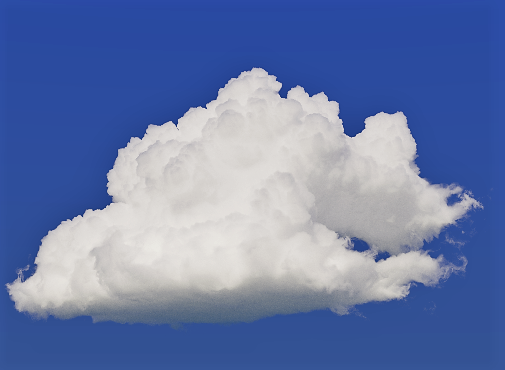
\includegraphics[width=\textwidth]{RaytracedCloud}
\end{figure}

\section{Custom heuristics}\label{sec:heuristics}
TODO: Describe heuristics currently used in games. Show that because of the hard time limits, the quality suffers greatly. Key articles: "Horizon Zero Dawn", "Battlefield"
\begin{figure}[!h]
    \caption{Clouds of Horizon: Zero Dawn}\label{fig:HorizonZeroDawn}
    \centering
    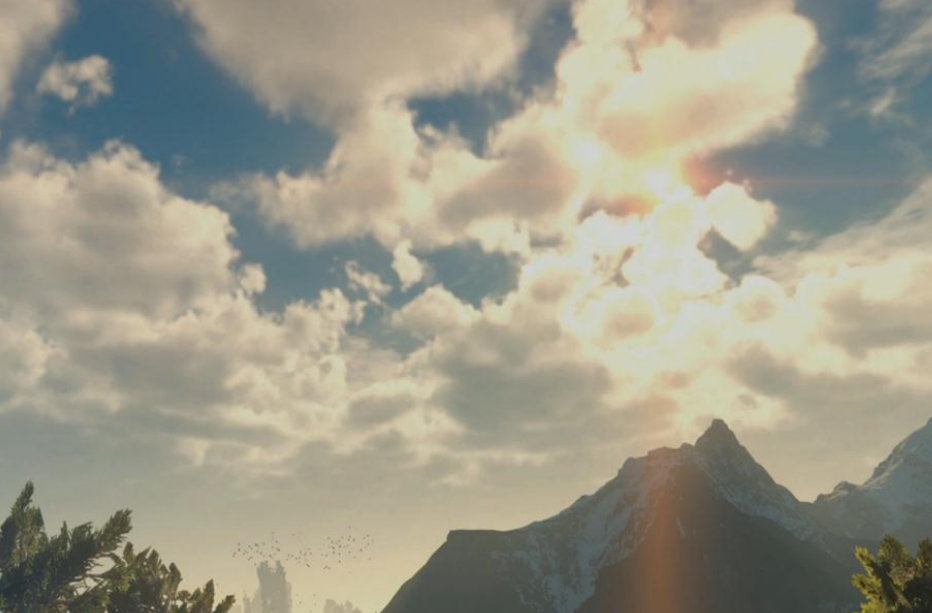
\includegraphics[width=\textwidth]{HorizonZeroDawn}
\end{figure}

\section{Neural Networks}\label{sec:NeuralNetworks}
TODO: explain the approach and technique of "Deep Scattering"
%% Так помечается конец обзора.
\finishrelatedwork

\chapter{Rendering with a neural network}
\section{Light Rendering Equation}\label{sec:LightRenderingEquation}
TODO: derive the light rendering equation and explain the exponentially increasing time with each bounce for clouds rendering
\section{Predicting radiance with a neural network}\label{sec:PredictingRadianceWithNN}
TODO: describe how to use neural networks to mitigate the exponentialy increasing rendering time.

\chapter{Rendering with partially baked neural networks}
\section{Key Iidea}\label{sec:keyIdea}
TODO: describe the general idea of llight backing and it's problems
\section{Network Architecture}\label{sec:architecture}
TODO: describe the network architecture
\section{Baking}\label{sec:baking}
TODO: describe the baking process
\section{Rendering}\label{sec:rendering}
TODO: describe the rendering process
\section{Dataset Generation}\label{sec:generation}
TODO: describe how the dataset is generated
\section{Training}\label{sec:training}
TODO: describe how the NN was trained: parameters, loss function, ...

\chapter{Results}
TODO: compare new results with old ones (performance and quality)


\end{document}
